%=================
\chapter{Sprint 1}
%=================
In this chapter the first sprint is explained. In \autoref{sec:sp1:planning} 
the planning of the first sprint is explained, the design of sprint 1 is 
covered in \autoref{sec:sp1:design}. \autoref{sec:sp1:impl} descripbes the 
features implemented in this sprint, and \autoref{sec:sp1:test} consists of 
the results from the tests. The feedback the team has got from the customer 
during the sprint is listed in \autoref{sec:sp1:feedback}, and the evaluation 
of the first sprint is covered in \autoref{sec:sp1:eval}.


%------------------------
\section{Sprint Planning}
%------------------------
\label{sec:sp1:planning}
The first sprint was started with a sprint planning meeting September 14th. 
The team is planning to implement basic and fundamental parts of the 
\gls{utility}. The most basic functionality was chosen from the product 
backlog, in order to end up with a utility that can generate simple 
\Gls{lua} \glspl{dissector} by the end of the sprint. This is important so we can see that we 
understood the project, and that the chosen \gls{preprocessor} and 
\gls{parser} is suitable for the utility.

\subsection{Duration}
%--------------------
Sprint 1 started September 14th, and lasted until September 27th. To avoid
misunderstandings between our developers and the customer, we will have weekly
meetings to show what we have accomplished and discuss further development. 

\subsection{Sprint Goal}
%-----------------------
The overall goal of the first sprint is to create a preliminary design and
implement the core of the application. It will be possible to run it to
generate \Gls{lua} \glspl{dissector}, which can be used by \Gls{wireshark} users. The first
version will contain only the basic \gls{dissector} generating features, for example,
parsing \Gls{c} \glspl{struct} with basic data types as \glspl{member}. Also, some of the
preprocessing capabilities will be implemented, such as handling \gls{include}
directives. Basic support for configuration will be added.

\subsection{Back Log}
In the first sprint we will implement eight requirements. These are listed in \autoref{tab:sprint1req}.
The time table for the sprint can be seen in \autoref{tab:sprint1time}.

\begin{table}[!htb] \footnotesize \center
\caption{Sprint 1 Requirements \label{tab:sprint1req}}
\begin{tabularx}{\textwidth}{l X c c}
	\toprule
	& & \multicolumn{2}{c}{Hours} \\
	\cmidrule(r){3-4}
	User story & Req. and Description & Est. & Act. \\
	\midrule
	\hyperref[tab:req:stories2]{US07} & FR6-A: Command line shall support parameter for \Gls{c} \gls{header} file & \textbf{9} & \textbf{9} \\
	& Implementation & 2 & 5 \\
	& Design & 1 & 1 \\
	& Testing & 2 & 2 \\
	& Documentation  & 4 & 1 \\
	\addlinespace
 	\hyperref[tab:req:stories1]{US01} & FR1-A: Support basic data types: \gls{int}, \gls{float}, \gls{char}, \gls{boolean} &  \textbf{24}  & \textbf{21} \\
	& Implementation & 8 & 13 \\
	& Design & 4 & 4 \\
	& Testing & 8 & 4 \\
	& Documentation & 4 & 0 \\
	\addlinespace
	\hyperref[tab:req:stories1]{US02} & FR2-A: The \gls{dissector} shall be able to display simple \glspl{struct} & \textbf{28} & \textbf{25} \\
	& Implementation & 8 & 17 \\
	& Design & 4 & 1 \\
	& Testing & 8 & 6 \\
	& Documentation & 8 & 1\\
	\addlinespace
	\hyperref[tab:req:stories1]{US04} & FR3-A: The \gls{utility} shall support \gls{include} & \textbf{8} & \textbf{2} \\
	& Implementation & 2 & 0 \\
	& Design & 2 & 1 \\
	& Testing & 2 & 1 \\
	& Documentation & 2 & 0\\
	\addlinespace
	\hyperref[tab:req:stories1]{US05} & FR3-B: Recognize invalid values for a \gls{struct} \gls{member} & \textbf{11} & \textbf{8} \\
	& Implementation & 11 & 8 \\
	\addlinespace
	\hyperref[tab:req:stories2]{US08} & FR6-B: Command line shall support paramter for configuration file & \textbf{28} & \textbf{8} \\
	& Implementation & 8 & 4 \\
	& Design & 8 & 2 \\
	& Testing & 8 & 2 \\
	& Documentation & 4 & 0 \\
	\addlinespace
	\hyperref[tab:req:stories2]{US06} & FR4-A: Support valid ranges for \gls{struct} \glspl{member} & \textbf{30} & \textbf{15} \\
	& Implementation & 8 & 8 \\
	& Design & 6 & 3 \\
	& Testing & 8 & 3 \\
	& Documentation & 8 & 1 \\
	\addlinespace
	\hyperref[tab:req:stories1]{US03} & FR2-D: Recognize invalid values for a \gls{struct} \gls{member} & \textbf{22} & \textbf{15} \\
	& Implementation & 6 & 9 \\
	& Design & 4 & 4 \\
	& Testing & 8 & 2 \\
	& Documentation  & 4 & 0 \\
	\midrule
	& Total: & 108 & 95 \\
	\bottomrule
\end{tabularx}
\end{table}

\begin{table}[!ht] \footnotesize \center
\caption{Sprint 1 Timetable\label{tab:sprint1time}}
\begin{tabularx}{\textwidth}{X c c}
	\toprule
	& \multicolumn{2}{c}{Hours} \\
	\cmidrule(r){2-3}
	Description & Est. & Act. \\
	\midrule
	Design & 30 & 10\\
	\addlinespace
	Implementation & 44 & 65 \\
	\addlinespace
	Testing & 50 & 20\\
	\addlinespace
	Documentation & 36 & 3\\
	\midrule
	Total: & 160 & 98 \\
	\bottomrule
\end{tabularx}
\end{table}


%----------------------
\section{System Design}
%----------------------
\label{sec:sp1:design}
This section introduces the design goals we decided on, the preliminary overall
design, and the final system design after the first sprint. In
\autoref{sec:sp1:impl}, we describe how our implementation works and is to be
used.

\subsection{Preliminary Design}
%------------------------------
The following is a description of the preliminary design we had for our
\gls{utility}. We split our program into several parts, described in the
following paragraphs. Their relationship is explained in
\autoref{fig:sp1:design}.

\begin{figure}[!htb]
	\center
	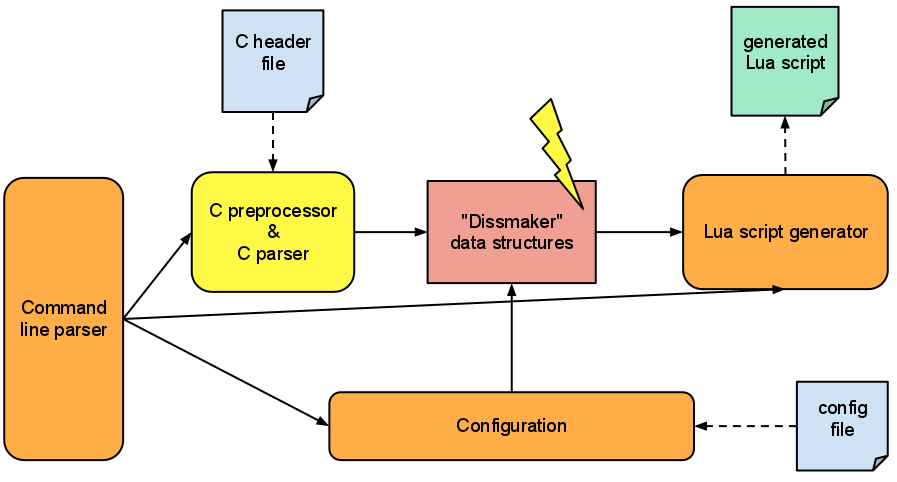
\includegraphics[width=\textwidth]{./sprints/img/design}
	\caption{Overall design\label{fig:sp1:design}}
\end{figure}

\paragraph{Command line interface}
The command line interface is where the user inputs which \gls{header} files and
configuration files he wants the \gls{utility} to use. This module needs to ask
the configuration to parse config files, and then ask the parser to parse \Gls{c}
files. It should finally ask the Lua script generator to create \Gls{wireshark} \glspl{dissector}
for the given \gls{header} files. The \gls{cli} should be able to accept some additional
arguments like verbose, debug, nocpp and output options.
The argument verbose should print out detailed information,
debug should print out debugging information, and nocpp should
disable the \Gls{c} \gls{preprocessor}. If the \gls{cli} is provided with invalid arguments, 
it should print a message explaining the correct usage.
If the program ran as expected it should output a message informing
the user of the success. 

\paragraph{Configuration}
The configuration should parse the configuration files given
to the command line interface, and from this information modify
the data structures generated by the parser.

\paragraph{Parser}
The most important part of the utility is the \gls{parser}, it should be able to parse \Gls{c} files and
look for \gls{struct} definitions. The \gls{struct} definitions will be put into a data structure
that the Lua script generator will use when creating the \glspl{dissector}.
The parser should use \gls{pycparser} and \gls{aply} \glspl{library} for parsing of \Gls{c} files. It should accept \Gls{c}
\gls{header} files and create an \gls{AST}, which is traversed
to find \gls{struct} definitions and their \glspl{member}. The \gls{struct} definitions and \glspl{member}
are then filled into a suitable data structure.

\paragraph{Data structures}
The data structures should store the information the Lua script generator needs to generate
\Gls{wireshark} \glspl{dissector}. It should have support for protocols and fields in \Gls{wireshark}.
The data structures should be easily modifiable by the configuration.

\paragraph{Lua script generator}
This is the part of the system that generates the actual \Gls{lua} \glspl{dissector}.
It should use the information in the data structures, from the 
parser and configuration, to create \Gls{lua} code that can dissect
the \gls{header} files specified by the user. 

\subsection{Utility}
%-------------------
Figure \ref{fig:sp1_class} illustrates the current class diagram for our
\gls{utility} after the end of the first sprint. The relationship between 
the modules can be seen in \autoref{fig:sp1_module}. The csjark module contains the main
method of the \gls{utility} and is responsible for running the program.
It is in this module we have implemented the functionality for the command line interface.

The \gls{utility} will typically start off by using cparser to parse the \Gls{c} \gls{header} file given to
the \gls{utility} as a command line argument. cparser will then use the config module
to ensure that the parsing is done correctly after the configuration, and then
generate protocols and fields to be used in the csjark module. The csjark
module then generates a \Gls{wireshark} \gls{dissector} in \Gls{lua} code by going through the
protocols and fields generated earlier by the cparser module.

In this sprint we added configuration support for ranges, this was done 
by adding a RangeRule class to the config module. This class specifies how
range rules should be written in the configuration. In the \gls{dissector} module
we created a RangeField class that interprets the rules
and recognizes any invalid values when generating the \glspl{dissector}.
The RangeField class inherits from the Field class.

\begin{figure}[!htb]
	\center
	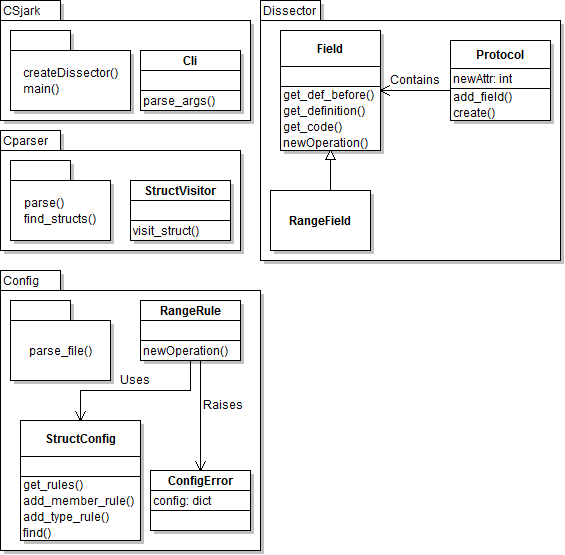
\includegraphics[width=\textwidth]{./sprints/img/ClassDiagramSprint1v2}
	\caption{Class Diagram\label{fig:sp1_class}}
\end{figure}

\begin{figure}[!htb]
	\center
	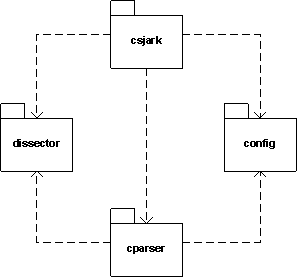
\includegraphics[width=0.50\textwidth]{./sprints/img/sp1modulediagram}
	\caption{Module Diagram\label{fig:sp1_module}}
\end{figure}

\subsubsection{Csjark}
%-------------------
The utilities \emph{main()} function is a part of the csjark module, the method will start parsing of CLI arguments, start parsing of the configuration files, and start generating dissectors by calling \emph{createDissectors()}. When all structs have been generated, it will print the results to the user on the command-line interface.

The Cli class will hold all the paramters, andl take the parameters from the command-line interface, it will parse the arguments and return lists for header and config.

\subsubsection{Cparser}
%-------------------
The Cparser module is used to parse the header files, and has three methods and a class. The preprocessing is done in \emph{parse\_file()}, \emph{parse()} is used to parse the file with pycparser library. To find a struct in the abstract syntax tree, the function \emph{find\_structs()} is used.

StructVisitor is a class that go through the abstract syntax tree, which the pycparser library generates. The class will handle all the declaration, and return a struct with the members.

\subsubsection{Dissector}
%-------------------
This module has three classes that generated the Lua dissector.

\begin{itemize}
	\item Protocol: This class generates the Lua dissector from a c struct. It will use Field class for each of the struct members.
	\item Field: Field is a class that generates code for each of the struct members. Field will used to generate code for basic data types, and will be a superclass for other data types and for fields that are configured.
	\item RangeField: Is a subclass of Field. It is modified in order to generate a field that will give a warning for an invalid value in Wireshark.
\end{itemize}

\subsubsection{Config}
%-------------------
This module consist of three classes, and a method to parse all the configuration files.
\begin{itemize}
	\item StructConfig: This is a class is used to store configuration for the c structs, and the configured members of the structs.
	\item RangeRule: This class is for range rules, stores information of minimum and maximum values, and the struct member.
	\item ConfigError: This class will raise an exception, if pyYAML is unable to parse the config file due to a error message.
\end{itemize}

%---------------------
\subsection{User Stories}
%---------------------
\label{sec:req:stories1}
This section lists the user stories for the first sprint. They are displayed in \autoref{tab:req:stories1} and \autoref{tab:req:stories2}.
As we are developing a very technical \gls{utility}, we have written user stories with an implementation level of abstraction. 
These user stories represent how we intend to add the functionality of each requirement to the \gls{utility}.
Each user story also contains information on how the modules of CSjark should interact with each other.

\begin{table}[htbp] \footnotesize \center
\caption{User Stories - Sprint 1 Part 1\label{tab:req:stories1}}
\noindent\makebox[\textwidth]{%
\begin{tabularx}{1.2\textwidth}{l X}
	\toprule
	Header & Value \\
	\midrule
	ID & US01 \\
	Requirements & FR1-A: The \gls{utility} should support the following basic data types: \gls{int}, \gls{float}, \gls{char} and \gls{boolean}. \\
	What & The administrator wants the \gls{utility} to support \glspl{struct} with \glspl{member} of basic data types in input files. 
		These are the basic data types in \Gls{c} that we support: \gls{int}, \gls{float}, \gls{char} and \gls{boolean}.\\
	How & The \Gls{c} \gls{parser} \gls{library}, pycparser, provides this support for us. The input is fed to the cparser module,
	which extracts the definitions from an \gls{AST} generated by the \gls{parser}.  \\
	Result & The \gls{utility} supports input with \Gls{c} \glspl{struct} with \gls{int}, \gls{float}, \gls{char} and \gls{boolean} \glspl{member}. \\
	\midrule
	ID & US02 \\
	Requirements & FR2-A: The \gls{utility} shall be able to display simple \glspl{struct}. \\
	What & The developer wants \Gls{wireshark} to display simple \glspl{struct}. \\
	How & The \gls{dissector} module shall generate \Gls{lua} \glspl{dissector} for Protocols created by the cparser module. 
		The \Gls{lua} \glspl{dissector} shall use \Gls{wireshark}'s API to display \glspl{struct} with basic \glspl{member}. \\
	Result & Simple \Gls{c} \glspl{struct} can be dissected in \Gls{wireshark} by our auto generated \Gls{lua} \glspl{dissector}. \\
	\midrule
	ID & US03 \\
	Requirements & FR2-D: Recognize invalid values for a \gls{struct} \gls{member}. \\
	What & The developer wants \Gls{wireshark} to give a warning if a \gls{struct} contains invalid values. \\
	How & The \glspl{dissector} module will generate fields that will display warning in \Gls{wireshark} when the value is 
	outside the configured range. \Gls{wireshark} will change the background color to yellow for fields with an invalid value, 
	and give an error message. \\
	Result & The developer can see when a value is out of range. \\
	\midrule
	ID & US04 \\
	Requirements & FR3-A: The \gls{utility} should support \gls{include}.\\
	What & The administrator wants the \gls{utility} to support the \gls{include}-statement inside a \gls{header} file.\\
	How & The cparser module feeds the input into an external tool, the \Gls{c} \gls{preprocessor}, which supports 
		\gls{include}-statements. It returns a \Gls{c} code file with all the included code from the external files. \\
	Result & The \gls{utility} supports \gls{include}. \\
	\midrule
	ID & US05 \\
	Requirements & FR3-B: The \gls{utility} should support \gls{define} and \gls{if}. \\
	What & The administrator wants the \gls{utility} to support \gls{define}- and \gls{if}-statement inside a \gls{header} file.\\
	How & The cparser module feeds the input into an external tool, the \Gls{c} \gls{preprocessor}, which supports 
		\gls{define}- and \gls{if}-statements. It returns a copy of the file with the statements removed, and their actions performed. \\
	Result & The \gls{utility} supports \gls{define} and \gls{if} functionality. \\
	\bottomrule
\end{tabularx}}
\end{table}

\begin{table}[htbp] \footnotesize \center
\caption{User Stories - Sprint 1 Part 2\label{tab:req:stories2}}
\noindent\makebox[\textwidth]{%
\begin{tabularx}{1.2\textwidth}{l X}
	\toprule
	Header & Value \\
	\midrule
	ID & US06 \\
	Requirements & FR4-A: Configuration must support valid ranges for \gls{struct} \glspl{member}. \\
	What & The administrator wants to be able to specify valid ranges for \gls{struct} \glspl{member} in a configuration file. \\
	How & The config module should read config files provided to the command line interface, and find any rules 
		regarding valid ranges. The rules are used by the cparser when it translates \gls{struct} definitions to Protocol 
		and Field instances found in the \gls{dissector} module. \\
	Result & The administrator can specify valid ranges of \gls{struct} \glspl{member} in the configuration.\\
	\midrule
	ID & US07 \\
	Requirements & FR6-A: Command line shall support parameter for \Gls{c}-\gls{header} file. \\
	What & The administrator wants the \gls{utility} to generate a \gls{dissector} from a \Gls{c}-\gls{header} file that he specifies.\\
	How & The command line user interface will accept a number of arguments from the administrator. The 
		argument that includes the path to an existing \Gls{c} \gls{header} file is sent to the \gls{parser} module. The parsing
		of arguments is done with the help of \gls{argparse} \gls{library}, which supports optional and positional arguments etc.\\
	Result & The command line interface supports \Gls{c}-\glspl{header} as input. \\
	\midrule
	ID & US08 \\
	Requirements & FR6-B: Command line shall support parameter for configuration file. \\
	What & The administrator wants to provide the \gls{utility} with one ore more configuration files. \\
	How & The command line interface should accept arguments that specifies the path of existing configuration
		files, and feed these to the config module. The config module should read the files and store them in configuration data 
		structures. These data structures will be available to cparser to help when translating \glspl{struct} to Protocol and
		Fields from the \gls{dissector} module. \\
	Result &  The administrator can input configuration files in the command line.\\
	\bottomrule
\end{tabularx}}
\end{table}


%-----------------------
\section{Implementation}
%-----------------------
\label{sec:sp1:impl}
In this sprint we have created a very naive implementation of the \gls{utility}. It
supports the most basic types of \Gls{c} \glspl{struct}. In addition, the \gls{utility} supports
some very basic configuration. The main reason for the naive implementation, 
was to find out that the \glspl{library} that the team had chosen, was suitable for 
the \gls{utility} and that we had understood the task.

To get a better understanding of how the different requirements were implemented,
look at the user stories for sprint 1 in \autoref{sec:req:stories1}.


\subsection{\gls{cli} Support for Header File}
%-------------------
The tool uses a command line interface. The user inputs a \Gls{c} \gls{header} file to the 
command line, and the program outputs a \Gls{wireshark} \gls{dissector} written in \Gls{lua}. 
Below you can see a \autoref{fig:sp1cmd} that illustrates how the program is 
run. 

\subsection{Support Basic \Gls{c} Data Types}
%-------------------
In this first sprint the focus was to generate \glspl{dissector} from \glspl{struct} with 
basic datatypes. These datatypes included \glspl{integer}, \glspl{float}, \gls{char}, \gls{boolean} and 
\glspl{array} of \glspl{char}. All different types of \glspl{integer} and \glspl{float} were also 
implemented in the \gls{utility}, most of the functionallity was included in the 
\gls{pycparser} \gls{library}, and sizes for the different data types was specified in the 
\gls{utility}.

\subsection{Display Simple Structs}
%-------------------
The \glspl{dissector} that our \gls{utility} generates is used to display the \glspl{packet} that 
are captured by wireshark. \autoref{fig:sp1wsstruct} shows an example of a 
\gls{packet} capture. The example include a \gls{struct} that is used to test different 
basic data types, for example, signed \gls{char}, \gls{char}, short, \gls{int}, long \gls{int}, \gls{float} 
and \gls{double}.

\begin{figure}[ht]
	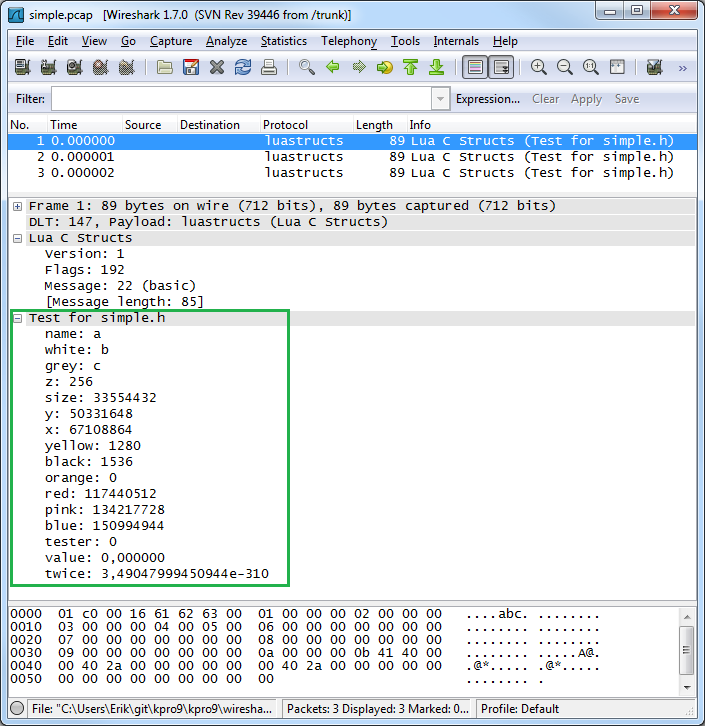
\includegraphics[width=\textwidth]{./sprints/img/wireshark_simple}
	\caption{Wireshark: Simple Lua dissector\label{fig:sp1wsstruct}}
\end{figure}

\subsection{Support \gls{include}}
%-------------------
The \gls{preprocessor} in \Gls{c} is the first step of compilation. One of the most used 
\gls{preprocessor} directives is \gls{include}, which include the content of a file 
in the compilaton. Since the \gls{utility} reads \glspl{struct} from \gls{header}-files, it is 
possible that \gls{struct} \gls{member} may have been defined in other \gls{header}-files, 
therefore \gls{include} is a important part of the \gls{utility}. The \gls{preprocessor} in 
this \gls{utility} will replace the \gls{include}-line with the content of the included file.

\subsection{Support \gls{define} and \gls{if}}
%-------------------
These two \gls{preprocessor} directives are important for our \gls{utility}. \gls{define} is 
used to define a \gls{preprocessor} macro that replaces a token with a 
sequence of characters. This can for example be used to define length of 
\glspl{array}, define values for enumeration or define a platform. \gls{if} and \gls{ifdef} 
are conditional directives that the \gls{utility} will use to check if macros are 
defined. This will be used when the \gls{utility} is generating \glspl{dissector} for 
different platforms. The functionallity for these \gls{preprocessor} directives and 
the other \gls{preprocessor} directives for \Gls{c}, was implemented by the \gls{library} we 
use, which is cpp.exe for \Gls{Windows} and \gls{agcc} for \Gls{mac} and \Gls{linux}.

\subsection{\gls{cli} Support for Configuration File}
%-------------------
To be able to parse the configuration file, it is necessary to specify the 
configuration-file in the \gls{cli}. An example of this is shown in 
\autoref{fig:sp1cmd}, where a \gls{header}-file and a config-file is input to the 
\gls{utility}. The option ''-v'' is specified, which will display the abstract 
syntax tree when the \gls{utility} has generated the \gls{dissector}.

\begin{figure}[ht]
	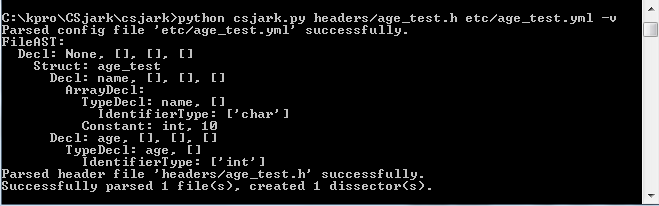
\includegraphics[width=\textwidth]{./sprints/img/cmd_agetest_run}
	\caption{Command line\label{fig:sp1cmd}}
\end{figure}

\subsection{Configuration of Valid Ranges}
%-------------------
We decided to use \gls{yaml} as our configuration format. In this sprint we have
added support for range specification. A user can specify the ranges of the
\glspl{member} of a \gls{struct}, from a minimum to a maximum. \autoref{code:rangesconf} 
shows an configuration in \gls{yaml} for the \gls{header}-file in \autoref{code:ranges}. 
The configuration specifes that the \gls{struct} \gls{member} age must have a value 
between 0 and 100.  

\lstset{language=C,caption={Configuration of valid ranges},label=code:rangesconf}
\lstinputlisting[language=C]{./sprints/code/ranges.yml}

\lstset{language=C,caption={Header-file for age\_test},label=code:ranges}
\lstinputlisting[language=C]{./sprints/code/ranges.h}

\subsection{Dissector Shall Recognize Invalid Values}
%-------------------
In \autoref{fig:sp1rangerule}, you can see how \Gls{wireshark} displays a \gls{member} that 
has an invalid range. When a invalid value exist, the \gls{dissector} will warn the 
user with a message and description, this make it easier for debugging.

\begin{figure}[htb]
	\center
	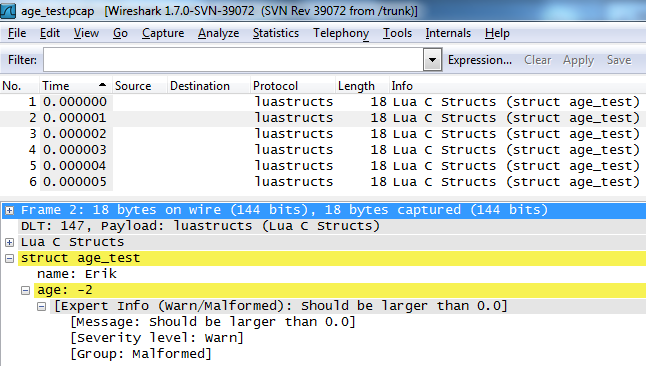
\includegraphics[width=\textwidth]{./sprints/img/wireshark_outofrange}
	\caption{\Gls{wireshark}: Invalid values\label{fig:sp1rangerule}}
\end{figure}


%-----------------------
\section{Sprint Testing}
%-----------------------
\label{sec:sp1:test}
This section introduces the tests preformed during the sprint and their
results.

\subsection{Test Results}
%-----------------
During the sprint the team executed a total of seven test cases. An example of a testcase run this sprint can be seen in \autoref{tab:STID01} while the rest of the test cases can be found in \autoref{sec:testcases}. These are the results for the tests the team ran for sprint 1 as according to \autoref{tab:testreport} discussed in the test plan.
The test results of the tests can be seen in \autoref{tab:sp1TIDS}.

\begin{table}[htb] \footnotesize \center
\caption{Test Case TID01}\label{tab:STID01}
\noindent\makebox[\textwidth]{%
\begin{tabularx}{1.2\textwidth}{l X}
	\toprule
	Header & Description \\
	\midrule
	Description & Supporting parameters for \Gls{c}-\gls{header} file \\
	Tester & Lars Solvoll Tønder \\
	Prerequisites & The utility must have been installed on the system and there needs to exist a header file associated with this test \\
	Feature & Test that we are able to feed the solution with a \Gls{c}-\gls{header} file and have it get dissected \\
	\midrule
	\multirow{2}{*}{Execution} & 1. Feed the utility with the name of the \Gls{c}-\gls{header} file associated with this test through the command line  \\
	& 2. Read the output given by the program \\
	\midrule
	\multirow{1}{*}{Expected result} & 2. The user should be presented with some text expressing the success of creating a dissector\\
	\bottomrule
\end{tabularx}}
\end{table}

\begin{table}[!htb] \footnotesize \center
\caption{Sprint 2 Test Results \label{tab:sp1TIDS}}
\noindent\makebox[\textwidth]{%
\begin{tabularx}{\textwidth}{l X}
	\toprule
	Header & Description \\
	\midrule
	Test ID & TID01 \\
	Description & Supporting parameters for \Gls{c}-\gls{header} file \\
	Tester & Lars Solvoll Tønder \\
	Date & 27.09.2011 \\
	Result & Failure. The \Gls{lua}-file got created successfully but the user was not informed of the result \\
	\midrule
	Test ID & TID02 \\
	Description & Supporting basic data types \\
	Tester & Lars Solvoll Tønder \\
	Date & 27.09.2011 \\
	Result & Failure. The program supports the use of \gls{int}, \gls{float}, \gls{char} and \gls{boolean}, but did not inform the user of the result\\
	\midrule
	Test ID & TID03 \\
	Description & Displaying simple \glspl{struct} \\
	Tester & Lars Solvoll Tønder \\
	Date & 27.09.2011 \\
	Result & Success\\
	\midrule
	Test ID & TID04 \\
	Description &  Supporting \Gls{c}-\gls{header} files with the \gls{include} directive  \\
	Tester & Lars Solvoll Tønder \\
	Date & 27.09.2011 \\
	Result & Failure. The program supports \gls{header} files with the \gls{include} directive, but did not inform the user of the result\\
	\midrule
	Test ID & TID05 \\
	Description &  Supporting \gls{define} and \gls{if}  \\
	Tester & Lars Solvoll Tønder \\
	Date & 27.09.2011 \\
	Result & Failure. The program supports \gls{header} files with the \gls{define} and \gls{if} directives, but did not inform the user of the result\\
	\midrule
	Test ID & TID06 \\
	Description &  Supporting configuration files  \\
	Tester & Lars Solvoll Tønder \\
	Date & 27.09.2011 \\
	Result & Failure. The program supports the use of configuration files but does not inform the user of any results\\
	\midrule
	Test ID & TID07 \\
	Description &  Recognizing invalid values  \\
	Tester & Lars Solvoll Tønder \\
	Date & 27.09.2011 \\
	Result & Success\\
	\bottomrule
\end{tabularx}}
\end{table}

\subsection{Test Evaluation}
%---------------------------
Most of our tests failed because the developers had forgotten to implement
usability features presenting the user with any textual information. With all
core functionality in place it only took three lines of code to fix this issue.


%--------------------------
\section{Customer Feedback}
%--------------------------
\label{sec:sp1:feedback}
This section covers the feedback we got from the customer before and after the first sprint.
Changes to the requirements are described in \autoref{sec:req:sprint4evo}.

\subsection{Pre-sprint}
%----------------------
The customer had no objections to the content of the first sprint, but was not
completely satisfied with the feature descriptions. They thought that we should
write more implementation details for each requirement, and that each
requirement should be properly broken down. They felt that
implementation and design should be two separate tasks if design is necessary.
Corollary to this, our work items were too big. They also suggested a proper
finish condition for each work item.

\subsection{Post-sprint}
%-----------------------
We presented the result from the sprint 1 for the customer and they were very
happy with the result. They had some ideas for how we could make our
configuration files more compact, but said that it was not really important.
Their other comments were mostly on what they wanted us to do for sprint 2
and how those features might be implemented.


%--------------------------
\section{Sprint Evaluation}
%--------------------------
\label{sec:sp1:eval}
This section contains the team evaluation of the first sprint.

\subsection{Review}
%------------------
The first sprint is over and the team has implemented a working \gls{utility} for simple structs. During
the sprint planning we decided which requirements from the product backlog that
we were to fulfill during the first sprint. The product backlog contains a
prioritized list of requirements. We decided to include the requirements that
had the highest prioritization. These requirements were basic, but essential
and therefore highly prioritized.
   
The lack of prior knowledge to \Gls{scrum} made planning and execution of the sprint
complicated for the team. We did not agree within the team of how to do it, and
wasted some time on discussions. In the end, we understood
that we wrote a too high level description of the requirements, and had to redo
previous work. This was time consuming, stealing person-hours from other parts
of the sprint.

Each requirement is divided in four parts: design, implementation, testing and
documentation. We currently have most of these parts covered, except
documentation for all files and unit test for the \gls{dissector} file. This work is
postponed till the second sprint.

The first sprint resulted in a solid core for our project. The customer was
happy with the first demo they got, the \gls{utility} even run on Mac.
 We feel that we have a good start and are confident
that we will be able to give the customer the product that they want in the
end.

The burndown chart, \autoref{fig:sp1:burndown}, shows the progress during
the first sprint. The team made an effort in making a correct estimation. This
is reflected in the chart, as the estimated and actual hours are  following
each other closely. In the end, actual hours stopped at 11 hours, which means we
have some uncompleted tasks. These are put back in the product backlog, and will
probably be part of the next sprint. 

\begin{figure}[!htb]
	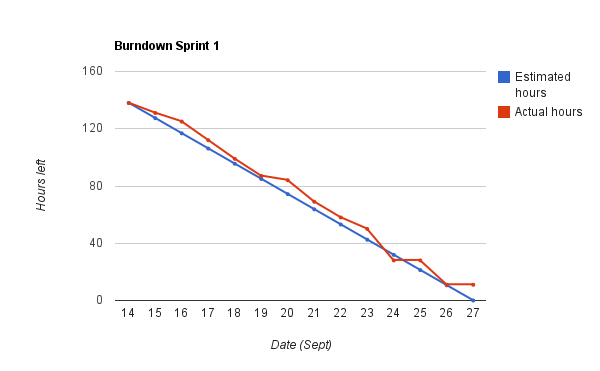
\includegraphics[width=\textwidth]{./sprints/img/burndown_chart_s1}
	\caption{Burndown chart\label{fig:sp1:burndown}}
\end{figure}

\subsection{Positive Experiences}
%--------------------------------
\begin{itemize}
	\item Good customer communication and relation from the beginning
	\item Implementation was easy
	\item Most of the requirements for this sprint were completed
	\begin{itemize} 
		\item all design, implementation and testing were completed
		\item documentation had to be put back in the product backlog 
	\end{itemize}
	\item Errors and bugs were detected and corrected swiftly and with relative ease
	\item The team functioned well, with sufficient discussions and conflicts
\end{itemize}

\subsection{Negative Experiences}
%--------------------------------
\begin{itemize}
	\item Hard for the team member to ''give'' 25 person-hours each week
	\begin{itemize}
		\item to understand that it is needed
		\item to free up so many hours, and still have time to do other subjects
	\end{itemize}
	\item Hard to find time for meeting/work where all team member was able to meet
	\item One member of the team was sick for a week
	\item We did not document the process and work during the first sprint well enough, which was a burden at the end of the sprint
	\item We did perhaps not understand \Gls{scrum} properly, which resulted in extra work
\end{itemize}

\subsection{Planned Actions}
%---------------------------
Below there is listed planned actions for the following sprints.

\subsubsection{Better Sprint Planning}
In order to avoid having to redo much of the work because of incorrect/poorly
sprint planning, we have decided to do this properly next time. We have learned
what we need to have in place and how to document it from this sprint.

\subsubsection{Design Early in the Sprint} 
The design should be in place early in the sprint. This is related to better
sprint planning, the planning should be so detailed/good that additional design
is not necessary. This is important for understanding and being able to
estimate hours and divide work.

\subsubsection{Documenting in Parallel while Implementing}
We suffered from the problem, code first then document. This is not a good
practise in team divided work. We will try to do the documentation as we code.
The documents for the project report also experienced a standstill while the
team worked on implementation. Writing parts of sprint documentation while
having the sprint is a much better way to work, then most part of the
documentation is already done before the sprint evaluation.

\subsubsection{Split Coding and Report Writing Between Team Members} 
Not all the team members have to do coding. It is important to maintain a
steady progress making the project report, while doing the implementation. 
Responsibilities for coding and report will be assigned next sprint. 

\subsection{Barriers}
%--------------------
Some of the team member have experienced some technical difficulties with their
Git client, and others had problems setting up PyCharm. Problems rose as we
realized that it would be hard setting up the programs on different
platforms.

We had problems with \Gls{c} \gls{parser} \gls{library}, \gls{pycparser}, which did not support \_Bool
type, specified in the \GLS{C99} standard. A patch for this was written by Even, and
was later included in the \gls{pycparser} \gls{library}. There was also problems with the
testing framework, attest, this framework did not have support for Windows
command line prompt, a patch was written and was later added to their \gls{library}.

Some team members had conflicting deadlines for deliveries in different courses.

